\chapter{Common solutions}
In this chapter we will try to summarize the most common techniques for solving the rendering equation in the presence of participating media. Many methods are used today and it's way beyond the scope of this thesis to do a proper summary of them, so only widely used methods related to the context of this thesis were picked.
\section{ Rasterization}
Rather than talking about game solutions, where is the main goal to render everything real time and physical accuracy of lighting is less important than plausible smooth graphics, we will have a look on rasterzation used in off-line rendering.
\\
\\
Rasterization comes as a nature choice, when it comes to particle rendering. It's key benefit is that the whole scene geometry doesn't have to fit into the RAM \footnote{Computer main random access memory.}, in the cost of linear rendering complexity. Because list of primitives, be it points, lines or triangles, is rasterized one by one in the frame-buffer.

\begin{minipage}{\linewidth}
      \begin{minipage}{0.45\linewidth}
          \begin{figure}[H]
              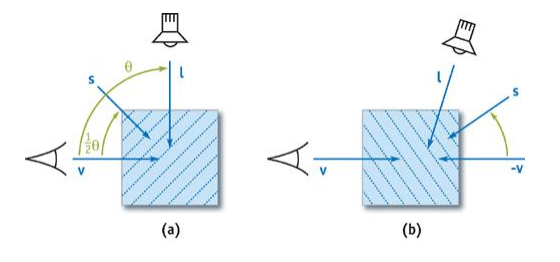
\includegraphics[width=\linewidth]{images/halfanglenvidia.png}
              \captionsetup{width=\linewidth}
              \caption[Half axis angle particle sorting and rendering.]{Illustration of the half axis angle determination for single particle sorting pass. Source \cite{NVIDIA}.}\label{fig:HAA}
          \end{figure}
      \end{minipage}
      \hspace{0.05\linewidth}
      \begin{minipage}{0.45\linewidth}
          \begin{figure}[H]
              \includegraphics[width=\linewidth]{\cestaImg nvidiasmokeparticles.jpg}
              \captionsetup{width=\linewidth}
              \caption[Nvidia smoke particle demo. Source \cite{NVIDIA}.]{This image has been rendered using multiple shadow maps for particle direct illumination on gpu. Source \cite{NVIDIA}.}\label{fig:NVS}
          \end{figure}
      \end{minipage}
  \end{minipage}
  \\
  \\
 \noindent{
Almost all the algorithms widely used rely on the same kind of preprocessing stage. The particles should be ideally sorted from the furtherest to the closest, and rasterized in this order, so that the alpha blending works correctly. Which is quite costly, considering we should sort millions of particles twice. Once for the camera view and once for the shadow map generation light view. To partially overcome this issue a half-angle axis sorting can be used, where we sort particles along a half angle axis between the camera and the light only once as can be seen on fig. \ref{fig:HAA}.
}
\\
\\
Also shadow map containing only a nearest depth is practically useless when used with millions of partially transparent particles. To cope with this we can either rasterize the particles in the common layer batches for camera view and light view to sample progressively reducing transmittance as used in nVidia demo fig. \ref{fig:NVS}. 
\\
\\
Or we can eventually use deep shadow maps \cite{LokDSM}, where is the occlusion function of depth\footnote{The function is usually represented as lookup table containing [depth,transmittance] tuples.} instead of a single value per pixel in the case of regular shadow maps. This approach allows pre-filtering\footnote{Object can occlude only partial part of the pixel, thus adding only appropriate amount of occlusion in incident depth.} which leads to suppression of both depth and aliasing artifacts commonly seen in shadow map renderings.
\\

\noindent{
Even tough only single scattering volume interaction can be modeled this way, it's very popular method widely used in the VFX industry, because it can handle very efficiently even billions of particles as can be seen on fig. \ref{fig:KRAK}. 
}

\myFigure{0.95}{\cestaImg krakatoa.jpg}{Krakatoa particle and volume rendering.}{Examples of rasterization Krakatoa particle render used in feature film productions \cite{KRAK} .}{fig:KRAK}

\section{Raytracing}
Another very popular set of methods for solving rendering equation is based on ray-tracing. Instead of rasterizing (drawing) directly visible elements, concept of ray scene interaction is used, where set of rays originating either in camera or in light are shoot into the scene space to gather light information. Which is way more flexible than rasterization, in the terms of complex light scene interaction and logarithmic cost of visibility computation\footnote{Not all the elements of the scene have to be usually intersected. And the complexity of ray element intersection in the present of volume partitioning acceleration structure such as KD or BVH tree is logarithmic.}.
\\
\\
The flexibility unfortunately goes in hand with an additional cost of acceleration structure build and usage for a ray primitive intersection. That's why these algorithms are so memory demanding. Because majority of the scene has to be loaded in the RAM for efficient visibility calculation.
\\
\\
In the following subsections the key ray-tracing concepts and methods are briefly overviewed.  

% great page for latex equation typing http://www.codecogs.com/latex/eqneditor.php
%Quasi Monte Carlo equation
%\begin{equation*}
%\int _{I^{S}}f(x)dx\approx\frac{1}{N}\sum_{i=1}^{N}f(x_{i})),
%\end{equation*}
%\int _{I^{S}}f(x)dx\approx\frac{1}{N}\sum_{i=1}^{N}f(x_{i})),

\subsection{Visibility evaluation}
The key aspect of ray-tracing volumes is the radiance integration between two points in space. Without the participating media the visibility is only a matter of ray surface intersection, the first object intersected by the ray is simply considered visible. In the presence of participating media we have to also consider transmittance change along the ray and in-scattered radiance along the path. For now we will stay with the transmittance evaluation only. In homogeneous media a simple analytic solution exists. Since $\kappa_t$ is constant we just evaluate the $  \tau(x_{0},x)=e^{-\kappa_t*\left | x_{0}\rightarrow x \right |}$.
\\
\\
In order to compute transmittance in non-homogeneous media according the eq. \ref{eq:TAU}, we can use ray-marching technique. Which evaluates the extinction coefficient of the media $\kappa_t(x_{v})\text{, in a point }x_{v}=\vec{r}*v$, where $\vec{r}$ is a ray direction and $v$ is some chosen step size. Ideally we should choose very small $v$, which would inevitably lead to render time increase. This technique also introduces bias to our estimate, which is not desired.
\\
\\
%tohle patri spis do pravdepodobnosti scateringu freeflyght distance ale tvrdi ze tak pocitaji transmitanci, je tam adaptive stepp size
Another technique used is known as Woodcock tracking \footnote{ The idea was used in neutron transport theory under different names mainly as delta tracking. Nevertheless Woodcock tracking is used in CG community to promote the original author.}. The idea is quite simple, if we know the maximum extinction coefficient of our media (which we very often know) we could sample the media randomly according to this coefficient more densely then needed. This approach is based on the probability theory behind the light particle interaction. To take steps according the transmittance probability density function, which is exponential function (eq. \ref{eq:TAU} ) we can sample according to it's inverse:
\begin{equation}
cdf(r)=-ln(1-r)/\kappa_\text{max}
\end{equation}
, where r is a uniformly distributed random variable and $\kappa_\text{max}$ is maximal extinction coefficient.

% ============ Unbiased methods =============

\myFigure{0.55}{\cestaImg temp.jpg}{Unbiased ray-tracing methods.}{Examples of unbiased ray-tracing methods, from left \ita{path tracing, light tracing, bidirectional path tracing}. The principle is pictured on the top raw and example renderings are in the bottom one.}{fig:UNBRT}

\myFigure{0.55}{\cestaImg temp.jpg}{Importance sampling function based on arbitrary pdf.}{Underlying density we try to estimate is represented as red function, our presumed probability distribution function is blue and generated samples are green vertical lines. As you can se when the right pdb is chosen samples are generated more densely in the areas of high function values and less in the areas of low function contribution. }{fig:IMPORTSAMPLING}

\subsection{Monte Carlo Ray-tracing}
Monte Carlo (from now on, abbreviated to MC) methods are commonly used for solving rendering equation, because robust analytical solution to the integral equation is not known. Since MC methods are based on numerical integration using random sampling and we can't integrate infinitely, these methods leads us to an approximate solution. The error introduced by the lack of samples is called variance and exhibits itself as a noise in the rendered image. The main benefit is that the convergence to the ground truth solution is independent on the problem domain and variance decreases linearly\footnote{Reduction rate is $(\frac{1}{n})$, where $n$ is number of samples}, the down side is that the standard deviation decreases in a $\frac{1}{\sqrt{n}}$. This means that, in order to half the noise level in the image, we have to generate four times more samples.
\\
\\
Many optimization steps can be taken to speed up the convergence. Some most used techniques are based on right choice of scene radiance sampling. The uniform distribution random samples might not be exactly what we are looking for, because the image is represented in the form of the uniform grid of pixels. Uniform sampling usually results in sample clumping in certain areas and we would ideally prefer to generate samples more evenly, but still randomly. To cope with this Quasi Monte Carlo sample generation and stratified sampling can be used for more uniform ray distribution. Some of the mentioned concepts can be used for sampling the brdfs and phase functions too. 
\\
\\
Other methods are based on importance sampling. This strategy distributes samples according to given probability density function (pdf) which should be as close as possible to the actual unknown density we try to estimate (fig \ref{fig:IMPORTSAMPLING}). As stated before these techniques don't guarantee any speedup. Choice of pdb can either make our sampling more efficient or totally ruin it. In practice though, the importance sampling plays major role and is key component of fast and accurate estimation.


\subsection{Path tracing}
Since the elements directly seen by the camera usually participate into the image most, concept of reverse radiance gathering from camera path to light is most popular Monte Carlo method of evaluating rendering equation. 
\\
\\
In its original form ray is recursively traced trough the scene and it's path is affected with scattering in the participating media and with refraction, refraction on surface hits until it reaches light source. After that, the light energy is weighted with accumulated probability and contribution sample added to the final image. 
\\
\\
Without a termination criteria the ray would travel infinitely, unfortunately fixed number of ray interaction events would introduce unwonted bias. Technique called Russian roulette is used to decide, whether to terminate the ray or let it continue it's
\\
\\
The popularity of path tracing is based two fact. It's quite simple algorithm that can be easily extended to support participating media, multiple light scattering and other effects, while it's guaranteed that it converges to ground truth result in the limit. The only down side of this approach is that it's computationally demanding process, sometimes many thousand rays per pixel have to be traced to obtain acceptable image with low noise level.
\\
\\
Unfortunatelly path tracing is not very effitient in rendering caustics because the probability of hiting light source trough multiple diffuse specular reflection is almost zero.




\subsection{Light tracing}
Is a dual algorithm to the path tracing. Paths are generated on the light sources and recursively traiced through the scene, when the sourface is hit or volume scattering event happens, shadow ray is casted to the camera. When the interaction point is unocluded on the path to camera, it gets projected and it's radiance value is added to the final image. 
\\
\\
This algorithm can be very inefective in large scenes where the majority of the paths never reaches the camera. Further more it fails to capture objects visible trough refraction because the probability that the ray will pass multiple refractions right to the camera is quite low. On the other hand light tracing can be used on small scale scenes for indirectct illumination accuracy evaulation purpouses, because it's unbiased and renders both surface and volume caustics much more efficiently than path tracing. See fig. \ref{fig:UNBRT} for the path tracing and light tracing algorithm comparison.


\subsection{Bidirectional methods}
This method tries to combine benefits of both path and light tracing methods. Rays are shoot from both camera and light and new light paths are generated as a result of their connection. To spedup the high energy path search and sampling, more elaborate methods like Metropolis light transport \cite{Veach97metropolislight}, do exist. These methods generate new paths using mutation of already found high energy paths.
\\
\\
However all these methods still fail to render specular reflection, refractions of caustics. This is caused by the fact that the probability of light reflecting of connecting a point on a specular surface to the camera results in zero contribution to the image.
\\
\\
Even though the convergence of bidirectional path tracing is much better than in the case of path and light tracing alone, many thousand rays are still needed to obtain noise free results.


% ============ Biased methods =============

%\subsection{Biased methods}

\subsection{Photon mapping}
Photon mapping is two pass method, first introduced by Jensen in the \cite{Jensen:1996} paper. It's loosely based on a bidirectional Monte Carlo ray tracing. Instead of direct light - camera path connecting, the flux carrying light paths of length at least two are cached in the form of so called "photons". These imaginary particles are shoot in the first pass of the algorithm and end up in one of the two photon map acceleration structures. Caustic photon map holds photons created by direct specular reflection/refraction paths from light. Or they end up in the indirect photon map structure, which holds photons after an interaction with the diffuse surface.
\\
\\
In the second rendering pass the camera rays are shot. The direct lighting component is
evaluated just like in the case of distributed ray tracing, but the indirect lighting is evaluated
using e photon maps. The caustic photon map is evaluated directly, because caustic effects
usually exhibit strong sharp features, while the slowly changing indirect lighting is evaluated
using final gathering the indirect photon map.


\subsection{Irradiance mapping}
\cite{jarosz08thesis} %jarosz thesis irradiance caching
irradiance caching, Photon tracing, final gather ...
Plus and cons



In the second rendering pass the camera rays are shot. The direct lighting component is evaluated just like in the case of distributed ray tracing, but the indirect lighting is evaluated using e photon maps. The caustic photon map is evaluated directly, because caustic effects usually exhibit strong sharp features, while the slowly changing indirect lighting is evaluated using final gathering the indirect photon map.


